\chapter{Results}
\label{ch_results}

These are the results I found from my investigation.

Present your results in a suitable format using tables and graphs where necessary. Remember to refer
to them in text and caption them properly.


\section{Simulation Results}


\section{Experimental Results}

\subsection{Focal Length of Lens}

The measured focal length of the lens was measured to be 53mm. Figure \ref{fig:focal_length_experiemnt_result} shows the focused point formed after adjusting the lens to 5.3cm above the working surface.

\begin{figure}[H]
	\centering
	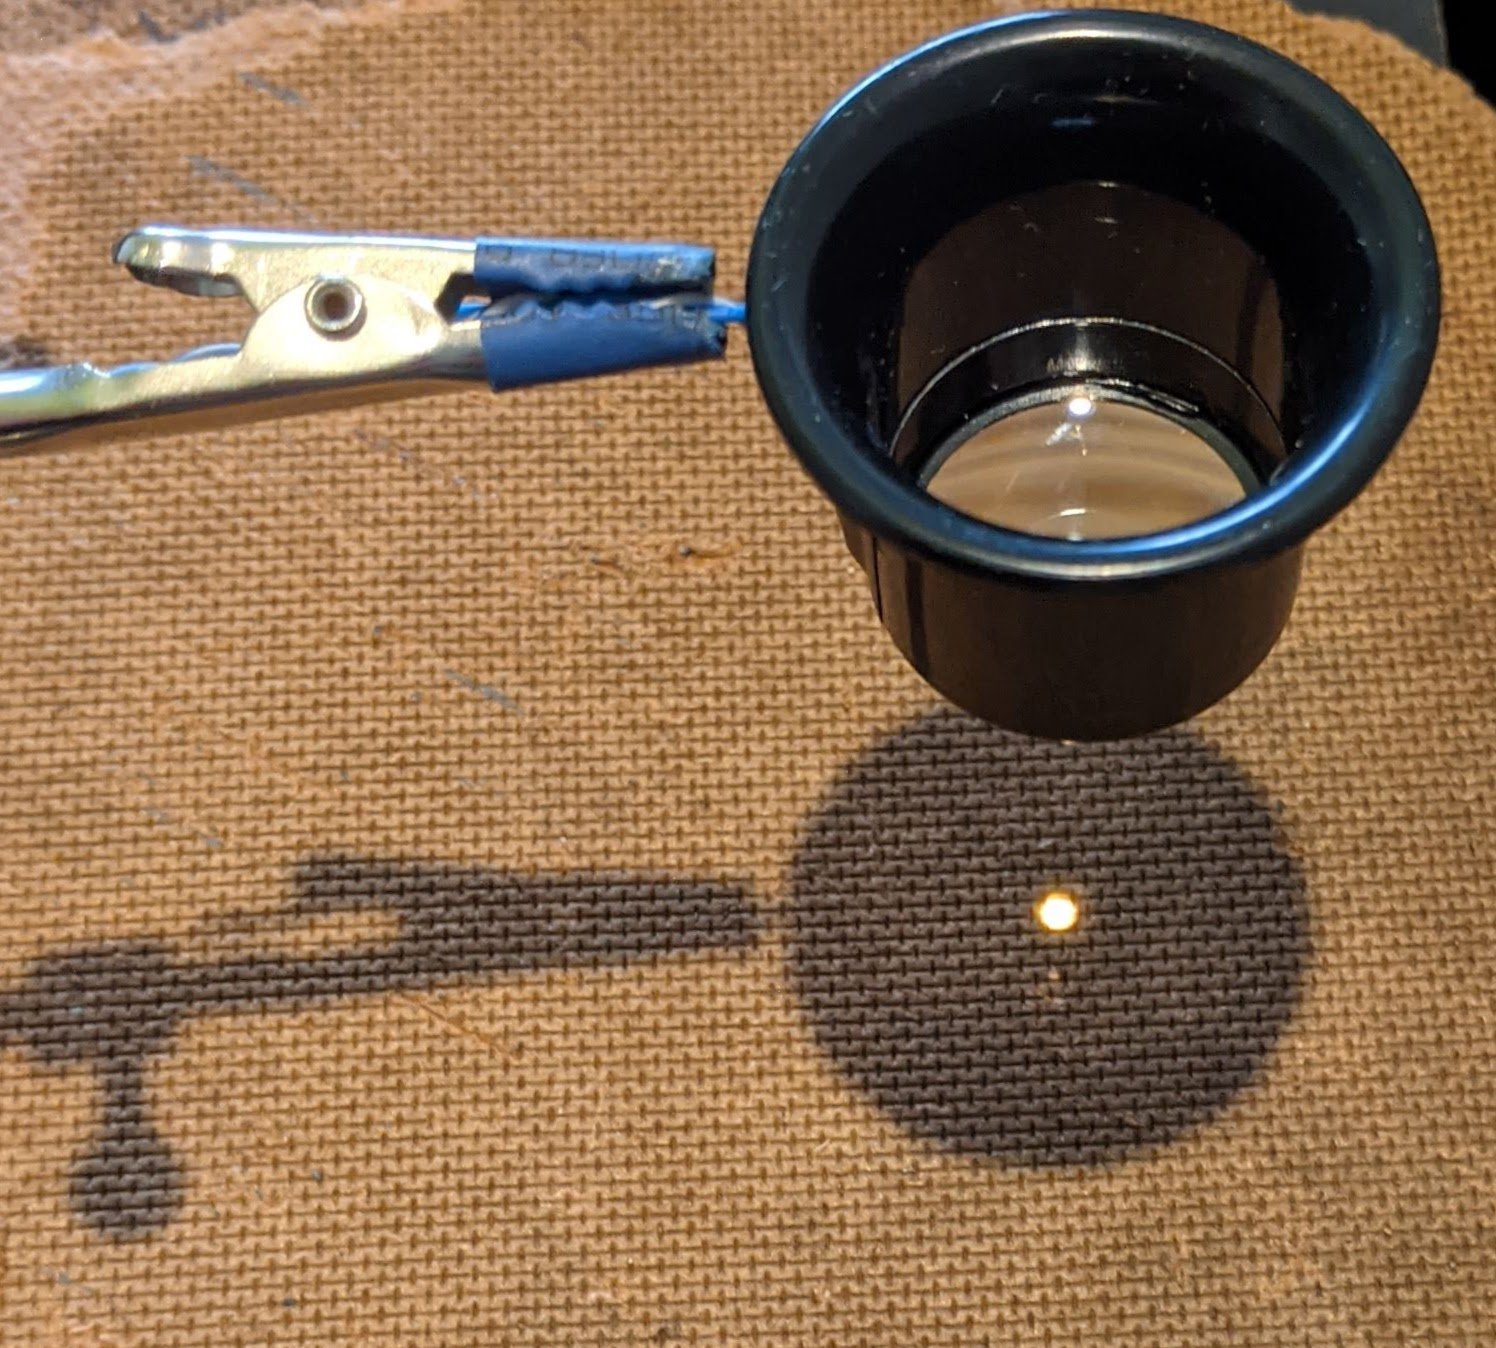
\includegraphics[width=.6\linewidth]{figures/results/focal_length_result.jpg}
	\captionof{figure}{Focal Length Experiemnt}
	\label{fig:focal_length_experiemnt_result}
\end{figure}


\subsection{Light Focus System}

Table \ref{label} below shows the beam spot size vs distance for the IR and warm-white power LEDs.

%table here